\documentclass[11pt]{article}

% ============================================================
% COMPILATION
% ============================================================
%
% Required compiler: XeLaTeX
%
% Recommended build sequence:
% XeLaTeX -> Biber -> XeLaTeX -> XeLaTeX
%

% ============================================================
% DOCUMENT EDITION
% ============================================================

\newif\iftutornotes

\tutornotestrue       % TA / Tutor edition
% \tutornotesfalse    % Student edition

% ============================================================
% PACKAGES
% ============================================================

\usepackage[a4paper,margin=1in]{geometry}

% XeLaTeX font system
\usepackage{fontspec}
\usepackage{unicode-math}

\setmainfont{TeX Gyre Termes}
\setsansfont{TeX Gyre Heros}
\setmonofont{Latin Modern Mono}
\setmathfont{TeX Gyre Termes Math}

\usepackage{microtype}
\usepackage{enumitem}
\usepackage{booktabs}
\usepackage{array}
\usepackage{longtable}
\usepackage{xcolor}
\usepackage{hyperref}
\usepackage{listings}
\usepackage{tcolorbox}
\usepackage{titlesec}
\usepackage{fancyhdr}
\usepackage[backend=biber,style=ieee]{biblatex}

% ============================================================
% DOCUMENT METADATA
% ============================================================

\newcommand{\CourseTitle}{Physical AI, TAICA}
\newcommand{\InstructorName}{Human-centered Intelligent System Lab}
\newcommand{\InstructorEmail}{National Yang Ming Chiao Tung University}

\newcommand{\AssignmentTitle}{Homework 1: 3D Scene Reconstruction}
\newcommand{\Semester}{Fall 2026}

% ============================================================
% BIBLIOGRAPHY
% ============================================================

\addbibresource{refs.bib}

% ============================================================
% TABLE SETTINGS
% ============================================================

\newcolumntype{L}[1]{>{\raggedright\arraybackslash}p{#1}}

% ============================================================
% HYPERLINK SETTINGS
% ============================================================

\hypersetup{
    colorlinks=true,
    linkcolor=blue!50!black,
    citecolor=blue!50!black,
    urlcolor=blue!50!black
}

% ============================================================
% PAGE STYLE
% ============================================================

\setlength{\headheight}{14pt}

\pagestyle{fancy}
\fancyhf{}

\lhead{\CourseTitle}
\rhead{\AssignmentTitle}
\cfoot{\thepage}

% ============================================================
% LIST SETTINGS
% ============================================================

\setlist[itemize]{
    topsep=3pt,
    itemsep=2pt,
    parsep=0pt,
    leftmargin=1.5em
}

\setlist[enumerate]{
    topsep=3pt,
    itemsep=2pt,
    parsep=0pt,
    leftmargin=1.6em
}

% ============================================================
% COLORS
% ============================================================

\definecolor{codebg}{RGB}{248,248,248}
\definecolor{commentgreen}{RGB}{0,110,60}
\definecolor{keywordblue}{RGB}{20,70,150}

% A single restrained color for all internal teaching notes.
\definecolor{tutorblue}{RGB}{65,88,110}
\definecolor{tutorbg}{RGB}{247,249,251}

% ============================================================
% TA / TUTOR NOTE SYSTEM
% ============================================================

% All material intended only for teaching staff may use this
% environment. Do not use separate teacher/grading/TA colors.
%
% In student mode, the complete environment body disappears.

\NewDocumentEnvironment{tutornote}{+b}
{%
    \iftutornotes
        \begin{tcolorbox}[
            colback=tutorbg,
            colframe=tutorblue,
            boxrule=0.4pt,
            arc=1mm,
            left=7pt,
            right=7pt,
            top=6pt,
            bottom=6pt,
            before skip=8pt,
            after skip=8pt
        ]
        {\small
        \color{tutorblue}
        \textbf{TA/Tutor Note.}\par
        \medskip
        #1}
        \end{tcolorbox}
    \fi
}
{}

% Optional edition indicator.
% It appears only in the teaching edition.

\newcommand{\EditionLabel}{%
    \iftutornotes
        \begin{center}
            {\small\color{tutorblue}
            TA / Tutor Teaching Edition}
        \end{center}
        \vspace{0.5em}
    \fi
}

% ============================================================
% LISTINGS
% ============================================================

\lstdefinelanguage{turtle}{
    alsoletter={:@},
    morekeywords={
        @prefix,
        a,
        owl:,
        rdf:,
        rdfs:,
        xsd:
    },
    sensitive=true,
    morecomment=[l]{\#},
    morestring=[b]"
}

\lstset{
    basicstyle=\ttfamily\small,
    backgroundcolor=\color{codebg},
    breaklines=true,
    frame=single,
    framerule=0.2pt,
    rulecolor=\color{black!20},
    keywordstyle=\color{keywordblue}\bfseries,
    commentstyle=\color{commentgreen},
    stringstyle=\color{black!70},
    columns=fullflexible,
    keepspaces=true,
    showstringspaces=false
}

\lstdefinestyle{codesnippet}{
    numbers=none,
    aboveskip=0.75\baselineskip,
    belowskip=0.85\baselineskip,
    frame=single,
    framerule=0.2pt,
    rulecolor=\color{black!20},
    backgroundcolor=\color{codebg},
    basicstyle=\ttfamily\small,
    breaklines=true,
    columns=fullflexible,
    keepspaces=true,
    showstringspaces=false
}

\newcommand{\code}[1]{\texttt{\detokenize{#1}}}

% ============================================================
% TITLE
% ============================================================

\title{\textbf{\AssignmentTitle}}
\author{
    \InstructorName\\
    \InstructorEmail
}
\date{\Semester}

% ============================================================
% DOCUMENT
% ============================================================

\begin{document}
\maketitle
\EditionLabel

% ============================================================
\section{Introduction}
% ============================================================
Imagine asking a household robot to bring you something from the kitchen. To do that safely, it needs a useful picture of the home: where rooms and furniture are, how spaces connect, and where it can move without collisions. A 3D scene map provides a spatial representation of the environment that can support navigation and scene understanding \cite{szeliski2022computer}.

\begin{figure}[htbp]
\centering
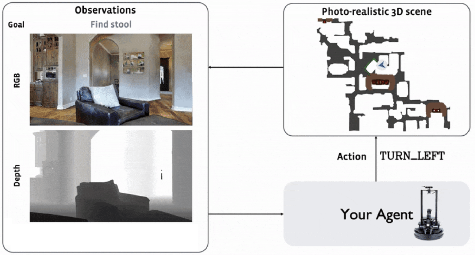
\includegraphics[width=0.78\linewidth]{image1.png}
\caption{Visual pipeline from RGB-D observations to a 3D scene.}
\label{fig:rgbd-to-scene}
\end{figure}

In this assignment, you will reconstruct apartment\_0, an indoor scene from the Replica dataset \cite{replica2019}, using RGB-D (color and depth) observations in Habitat-Sim \cite{habitatsim2020} simulator. The reconstruction pipeline converts depth images into 3D point clouds, registers observations from multiple viewpoints, integrates them into a unified 3D scene, and evaluates the result through visual inspection and comparison of the estimated camera trajectory with ground truth. In addition to reconstruction, you will examine the input observations to understand how conditions such as missing or noisy depth, insufficient viewpoint overlap, and large frame-to-frame motion relate to the resulting map and trajectory. Together, these components connect the characteristics of the input data with the behavior of the reconstruction process.
Although conducted in simulation, this assignment provides a starting point for considering the challenges involved in building and using 3D scene maps for real-world robotic tasks.

% In this assignment, you will reconstruct apartment\_0, an indoor scene from the Replica dataset \cite{replica2019}, using RGB-D (color and depth) observations in Habitat-Sim \cite{habitatsim2020} simulator. The reconstruction process converts depth images into 3D point clouds, registers point clouds captured from multiple viewpoints, and integrates them into a unified 3D scene. Reconstruction quality is assessed through visual inspection and quantitative comparison of the camera trajectory against ground truth. These steps form the core reconstruction pipeline.

%This is an enhanced version of the standard 3D reconstruction task: in addition to implementing the required Open3D pipeline \cite{open3dglobal}, you will verify the input data and use measurements to explain how capture conditions affect reconstruction. Missing or noisy depth, insufficient viewpoint overlap, and large frame-to-frame motion are among the failure conditions examined in this assignment.

%The assignment has two phases. Phase 1 uses a provided first-floor capture. Phase 2 uses the Habitat simulator (Habitat-Sim) \cite{habitatsim2020} to collect a second-floor capture yourself. Both phases use the same reconstruction and verification workflow, so you can compare a supplied capture with one shaped by your own navigation and collection choices.

%It consists of two phases. In Phase 1, you will reconstruct the first floor using the provided RGB-D observations. In Phase 2, you will navigate the second floor and collect your own RGB-D observations and camera poses. Both phases follow the same reconstruction and verification workflow, allowing you to examine how navigation and data-collection choices influence reconstruction outcomes.

% ============================================================
% \section{Learning Objectives}
% ============================================================
\vspace{1em}
By completing this assignment, you will be able to:
\begin{enumerate}
\item Understand the pipeline from RGB-D observations to 3D scene reconstruction, including the pinhole camera model, point-cloud generation, registration, mapping, and trajectory estimation.
% \item Understand how data quality and capture choices affect registration stability, scene quality, and reconstruction performance.
\item Analyze input observations and capture choices to identify factors associated with reconstruction behavior and failure cases.
% \item Evaluate and communicate reconstruction quality using data-verification evidence, visualizations, and the required Mean L2 Distance metric.
\item Evaluate and communicate reconstruction results using quantitative metrics, visualizations, and data-verification evidence.
\end{enumerate}

% ============================================================
\section{Structure and Workflow}

This assignment is organized into \textbf{two phases} that share the same reconstruction
and data-verification workflow. The main difference lies in how the input
observations are obtained:

\begin{itemize}
    \item \textbf{Phase 1:} Use a provided first-floor batch containing designed data-quality variations to reconstruct a 3D scene map, diagnose factors that contribute to reconstruction failures, and refine the reconstruction based
on the analysis.

    \item \textbf{Phase 2:} Extend the same workflow to the second floor, where you will collect your own RGB-D observations and camera poses through navigation in the simulation and reconstruct the scene from the collected data.
\end{itemize}

For the reconstruction component, the workflow follows the general registration
procedure described in the \textbf{Open3D}~\cite{open3dglobal} documentation, including
point-cloud downsampling, global registration, and local refinement. The results
from both phases are then compared to examine how data-collection choices and
observation characteristics relate to reconstruction outcomes.

%============================================================

\subsection{Reconstruction Pipeline}

The reconstruction work in both phases follows the pipeline below:

\begin{enumerate}
\item \textbf{Depth Unprojection.} Convert valid depth pixels to 3D points using the pinhole camera model. Use the resolution, field of view (FOV), and depth scale recorded in \code{intrinsics.json}. Implement this mapping yourself; \textbf{do not use Open3D projection functions
for this step.}
\item \textbf{Voxelization (Downsampling).} Reduce the number of points to improve computational efficiency while retaining the scene structure. Open3D functions may be used for this step\cite{open3dglobal}.
\item \textbf{Global Registration (RANSAC).} Estimate an initial alignment between point clouds to handle large viewpoint differences using the Random Sample Consensus (RANSAC)~\cite{fischler1981ransac}. Open3D functions may be used for this step~\cite{open3dglobal}.
\item \textbf{Local Registration (ICP).} Starting from the global-registration result, refine the transformation between
point clouds using the Iterative Closest Point (ICP)~\cite{chen1992object} algorithm. Open3D's point-to-point or point-to-plane ICP implementation may be used for this step~\cite{open3dglobal}.
\item \textbf{Scene Map Reconstruction and  Evaluation.} Transform and accumulate the aligned point clouds into a unified 3D scene map and construct the estimated camera trajectory. For clearer visualization, remove the ceiling when necessary, and visualize the estimated trajectory in red and the ground-truth trajectory in black. Evaluate the estimated trajectory against the ground truth using the required Mean L2 Distance. Open3D functions may be used for point-cloud processing, transformation, and visualization~\cite{open3dglobal}.
\end{enumerate}

After completing the reconstruction, evaluate the resulting scene and camera trajectory together with the \textbf{data-verification process}. If the reconstruction contains noticeable artifacts or alignment failures, identify likely contributing factors from the observations and reconstruction settings, adjust the relevant preprocessing or registration parameters, and rerun the pipeline as needed.

\subsubsection{Depth Unprojection}

% The reconstruction begins with synchronized RGB-D observations, each consisting of a color image and a depth image corresponding to the same camera viewpoint. The depth measurements are then back-projected into 3D using the camera intrinsics, while ground-truth (GT) poses, when available, are used only as references for trajectory evaluation. 

Each RGB-D observation contains a color image and a depth image corresponding to the same camera viewpoint. For reconstruction, each valid depth pixel is converted into a 3D point in the camera coordinate frame using the pinhole camera model. Given calibrated camera intrinsics $(f_x,f_y,c_x,c_y)$ and a valid stored depth value $D(u,v)$ at pixel $(u,v)$, the metric depth is first computed as $Z=D(u,v)/s$, where $s$ is the depth scale. The corresponding 3D point is then obtained by back-projecting the pixel into the camera coordinate frame~\cite{hartley2004multiple}:

% \[
% X=\frac{(u-c_x)Z}{f_x},\qquad Y=\frac{(v-c_y)Z}{f_y},\qquad Z=\frac{D(u,v)}{s},
% \]
% The symbols in this equation are annotated as follows:
% \[
% \begin{aligned}
% X,Y,Z &:\ \text{camera-coordinate components}, & u,v &:\ \text{pixel column and row},\\
% f_x,f_y &:\ \text{horizontal and vertical focal lengths (pixels)}, & c_x,c_y &:\ \text{principal-point coordinates (pixels)},\\
% D(u,v) &:\ \text{raw depth value}, & s &:\ \text{depth scale}.
% \end{aligned}
% \]
\vspace{-0.5em}
\[
X=\frac{(u-c_x)Z}{f_x},\qquad
Y=\frac{(v-c_y)Z}{f_y},\qquad
Z=\frac{D(u,v)}{s}.
\]

The symbols in this equation are annotated as follows:
\[
\begin{aligned}
X,Y,Z &:\ \text{3D coordinates in the camera frame}, & u,v &:\ \text{pixel column and row},\\
f_x,f_y &:\ \text{horizontal and vertical focal lengths (pixels)}, & c_x,c_y &:\ \text{principal-point coordinates (pixels)},\\
D(u,v) &:\ \text{stored depth value}, & s &:\ \text{scale from raw depth to meters}.
\end{aligned}
\]

Applying this unprojection to all valid depth pixels produces a point cloud for each RGB-D observation. These point clouds form the geometric input to the registration stage.

\subsubsection{Global and Local Registration}

Each point cloud is expressed in its own camera coordinate frame, so observations from different viewpoints cannot be directly combined. Registration estimates the relative transformations needed to align them in a shared coordinate system. Following the steps in Open3D document~\cite{open3dglobal}, the alignment is then performed in two stages: global registration with Random Sample Consensus (RANSAC)~\cite{fischler1981ransac} algorithm, and local refinement with Iterative Closest Point (ICP)~\cite{chen1992object} algorithm.

\vspace{0.5em}
\noindent\textbf{Global Registration.}
Global registration estimates an initial alignment between point clouds without requiring a close initial pose. The point clouds are first downsampled and represented using Fast Point Feature Histograms (FPFH)~\cite{rusu2009fast}, which provide local geometric descriptors for establishing candidate correspondences. Random Sample Consensus (RANSAC)~\cite{fischler1981ransac} then repeatedly samples candidate correspondences, estimates a transformation, and rejects inconsistent matches using geometric consistency checks. Only correspondences that pass these checks are used to estimate and validate the transformation. The resulting alignment provides a coarse global registration that can be further refined in the local-registration stage.

\vspace{0.5em}
\noindent\textbf{Local Registration.}
Local registration further refines the alignment between point clouds using Iterative Closest Point (ICP)~\cite{chen1992object}. Starting from an initial transformation, ICP repeatedly establishes correspondences between the source and target point clouds, estimates a transformation that reduces the alignment error, and updates the source point cloud. This process continues until the convergence criterion is reached. Open3D provides both point-to-point and point-to-plane formulations for ICP~\cite{open3dglobal}. Point-to-point ICP minimizes the Euclidean distance between corresponding points, whereas point-to-plane ICP minimizes the distance from each source point to the tangent plane defined by the corresponding target point and its surface normal. 

\vspace{0.5em}
After global and local registration, the estimated pairwise transformations describe the relative poses between point clouds. By choosing one point cloud as the reference frame and composing these transformations, the remaining point clouds can be transformed into the same coordinate system and accumulated to form a complete scene map. Registration performance depends on parameters such as voxel size, correspondence thresholds, and convergence criteria. Different settings may affect alignment quality, robustness, runtime, and ultimately the reconstructed scene. These parameter choices should therefore be examined and documented during the reconstruction process.

% The estimated transforms place aligned clouds in a shared coordinate system, where they are accumulated into a 3D scene map. The pipeline also composes an estimated camera trajectory, visualizes the map and trajectories, and evaluates the result against GT poses when available. The estimated trajectory may be shown in red and the GT trajectory in black; remove the ceiling from the scene visualization when it obstructs inspection.

\subsubsection{Scene Map Reconstruction and  Evaluation}

After registration, the aligned point clouds are accumulated into a reconstructed 3D scene, while the estimated pairwise transformations are composed to recover the camera trajectory. Reconstruction is evaluated through both visual inspection of the scene map and quantitative comparison of the estimated trajectory with the ground-truth (GT) trajectory. GT poses are used only for evaluation and are not used as inputs to the reconstruction process.

For quantitative trajectory evaluation, this assignment uses the \textbf{Mean L2 Distance}, defined as the mean Euclidean $L_2$ distance between estimated and ground truth camera positions. For $N$ evaluated frames, use:

\vspace{-1em}
\[
\operatorname{MeanL2}=\frac{1}{N}\sum_{i=1}^{N}\left\|\hat{\mathbf p}_i-\mathbf p_i^{\mathrm{GT}}\right\|_2,
\]
The symbols in this equation are annotated as follows:
\[
\begin{aligned}
N &:\ \text{number of evaluated frames}, & i &:\ \text{frame index},\\
\hat{\mathbf p}_i=(\hat{x}_i,\hat{y}_i,\hat{z}_i) &:\ \text{estimated camera position},\\
\mathbf p_i^{\mathrm{GT}}=(x_i^{\mathrm{GT}},y_i^{\mathrm{GT}},z_i^{\mathrm{GT}}) &:\ \text{ground-truth camera position},\\
\|\cdot\|_2 &:\ \text{Euclidean }L_2\text{ norm}.
\end{aligned}
\]
For each capture, the first camera pose defines the reference frame. The estimated trajectory is initialized in this frame, and the GT trajectory is transformed to the same frame for evaluation. This common reference frame is the shared scene coordinate system. A lower Mean L2 Distance indicates closer agreement between the estimated and ground-truth camera poses.

% The two phases apply this same pipeline to different floors of apartment\_0. Phase 1 uses the provided first-floor RGB-D data; Phase 2 uses second-floor RGB-D observations collected by students with a Habitat-Sim agent. Compare viewpoint coverage, frame spacing, overlap, registration choices, visual map quality, Mean L2 Distance, and runtime across the two reconstructions.

%============================================================

% \subsection{Technical Foundations}

% The following sections summarize the core concepts needed for the reconstruction and data-verification workflow. They introduce RGB-D scene reconstruction, the factors used for data verification, and the basic data structures used to organize the resulting evidence.

%============================================================

\subsection{Data Verification Pipeline}
Recent advances in AI have moved perception, prediction, and decision systems
from isolated demonstrations into products and services that influence the
physical world. As a result, it is no longer sufficient to report only an
output or a performance score: developers and users also need to inspect the
data and assumptions that led to that output. This need is particularly
important in Physical AI. A robot acts from time-varying sensor observations,
so missing depth, weak geometric support, or abrupt camera motion can affect a
downstream reconstruction even when the code itself is unchanged.

Raw PNG files, NumPy arrays, and terminal logs are useful but do not, by
themselves, state how an observation, a measurement setting, a verdict, and a
reconstruction run are related. This assignment therefore adds a
\textbf{semantic layer}: machine-readable descriptions placed above the raw
data. An \textbf{ontology} is a suitable foundation for this layer because it
defines shared classes, relations, and constraints rather than relying on
informal filenames or ad hoc notes. Here,
\code{ontology/hw1.ttl} defines the vocabulary for batches, frames, RGB and
depth images, quality factors, settings, annotations, frame pairs, and
reconstruction runs. The provided tools read this vocabulary as their
contract, so the same terms support both human explanation and programmatic
checks.

In this assignment, RDF represents verification evidence as triples, which are
stored together in a local triple store and written in readable Turtle files.
SPARQL queries that store by describing relationships among the triples, so
students and the reconstruction program can retrieve frames that meet the
declared verification criteria.

\begin{itemize}
\item \textbf{RDF (Resource Description Framework):} A standard way to
represent information as linked statements. Here, RDF describes captures,
frames, measurements, verification results, and reconstruction runs.
\item \textbf{Triple:} One RDF statement with a subject, predicate, and object.
For example, a triple can say that an annotation describes a frame or that its
status is \code{Pass}.
\item \textbf{Triple store:} A collection of RDF triples that can be searched
by their relationships. The assignment uses a local triple store, so no
database server is required.
\item \textbf{Turtle:} A compact, readable text format for writing RDF
triples. The ontology and each experiment's evidence are provided as
\code{.ttl} files.
\item \textbf{SPARQL query:} A query that retrieves information from RDF by
specifying patterns of relationships. Students use SPARQL to inspect
verification evidence and select qualified frames for reconstruction.
\end{itemize}

The semantic layer records provenance and makes a data-quality claim
inspectable; it does not prove that one factor caused a reconstruction outcome.
Use the evidence to form and test an explanation by comparing the whole-batch
and selected reconstructions. The workflow has three connected stages:
\emph{declare} an experiment and its factors, \emph{annotate} the raw data
with measured evidence, and use the recorded results to select frames for
reconstruction.
The command examples in this section assume that you run them from the homework
directory, \code{<repository-root>/hw1}.

\subsubsection{Declare an Experiment with Specified Factors}

An \textbf{Experiment} is one named verification condition for one capture
batch. Treat it as a small design-of-experiment statement: before computing
any result, state which data you will inspect, which quality factors matter,
which settings define a pass, and what you expect to observe. This prevents a
conclusion from being chosen after the measurements are known, and it makes
different verification choices comparable.

Selecting factors is part of this design. Each factor measures a different
possible condition in the data, and the selected factors define the evidence
that will be measured and later used to qualify frames. Choose factors that
test your hypothesis; selecting every factor without a reason makes the
experiment harder to interpret, while omitting a relevant factor leaves that
condition unexamined.

\code{api.py declare} is a helper that makes this declaration easy to start.
It creates a boilerplate Turtle file with the prefixes, experiment identifier,
batch link, selected-factor slots, setting guidance, and prediction prompts.
It does not measure the data or decide whether frames pass: those remain the
purpose of your experiment. Use it to create a new boilerplate for each
verification condition:
\begin{lstlisting}[language=bash]
pixi run -e habitat python api.py declare \
  --name <experiment-name> \
  --data-dir <capture-directory> \
  --floor <floor-number> \
  --factor <factor-name>
\end{lstlisting}

Repeat \code{--factor} for every selected factor. The helper creates a
boilerplate in \code{experiments/}, named
\code{<experiment-name>.ttl}. Review and complete it before assessment. Record
the factor selection and any setting changes there.

The available factors operate on one RGB image, one depth image, or an ordered
pair of consecutive depth images. They are diagnostic measurements for
inspection and interpretation; no single scalar predicts reconstruction success
or establishes causation. RGB exposure factors provide context about appearance
and feature visibility~\cite{shin2019camera}; ICP itself aligns
depth-derived point clouds~\cite{chen1992object}.

\begin{itemize}
\item \textbf{RGB-image factors}
    \begin{itemize}
    \item \code{HighlightClipping}: the fraction of pixels with a channel at
    an explicitly chosen high threshold. It records overexposure and provides
    context for feature visibility~\cite{shin2019camera}.
    \item \code{ShadowClipping}: the fraction of pixels whose channels all
    meet an explicitly chosen low threshold. It records underexposure and
    limited visible detail~\cite{shin2019camera}.
    \end{itemize}
\item \textbf{Depth-image factors}
    \begin{itemize}
    \item \code{HighFrequencyDepthResidual}: a robust local high-pass
    depth-noise estimate~\cite{immerkaer1996fast}; noisy points can disturb
    back-projection and local alignment.
    \item \code{FlyingPixelRatio}: the fraction of mixed-boundary depth
    returns; inconsistent boundary points can weaken geometric alignment.
    \item \code{ValidTileCoverage}: the share of fixed-size depth tiles with
    sufficient valid measurements; it describes the spatial distribution of
    usable geometry.
    \end{itemize}
\item \textbf{Consecutive depth-pair factors}
    \begin{itemize}
    \item \code{IdentityMedianDepthChange}: the median absolute depth change
    over jointly valid pixel coordinates; large change can signal a difficult
    pairwise alignment.
    \item \code{JointValidDepthRatio}: the fraction of pixel coordinates with
    valid depth in both images; it is a proxy for shared geometric support.
    \item \code{PriorWarpDepthResidual}: the median depth disagreement after
    warping one frame under a motion prior; it indicates disagreement with the
    predicted alignment.
    \end{itemize}
\end{itemize}

\subsubsection{Annotate Raw Data from the Selected Factors}

The declaration tells the verifier what to look for in the raw data. When you
assess it, the selected factors are measured on the corresponding RGB images,
depth images, or consecutive depth pairs. Their values and pass/fail results
become annotations attached to the experiment, so the raw observations now
carry recorded verification evidence.
\begin{lstlisting}[language=bash]
pixi run -e habitat python api.py experiment \
  experiments/<experiment-name>.ttl
\end{lstlisting}
The completed Turtle file is the evidence record for this experiment. Inspect
it with \code{api.py explore} when you need to see which observations passed or
failed. If you need a different factor selection or threshold, declare a new
experiment rather than changing the assessed record.

\subsubsection{How Verification Results Select Reconstruction Frames}

The annotations connect each measured value and status to its source frame or
frame pair. The reconstruction program reads these recorded results and uses
the default usable-link rule to form its selected frame sequence. The SPARQL
query below is an example of how such relationships can be queried; it is
provided to illustrate the semantic layer and is not an assignment deliverable.

\begin{lstlisting}[language=sparql]
PREFIX hw1: <http://taica.course/hw1/ontology#>

SELECT DISTINCT ?frame ?frameIndex
WHERE {
  ?experiment hw1:producesPair ?pair .
  ?pair hw1:sourceFrame ?source ;
        hw1:targetFrame ?target ;
        hw1:qualificationStatus hw1:Pass .
  FILTER NOT EXISTS {
    ?experiment hw1:producesAnnotation ?annotation .
    ?annotation hw1:annotatesFrame ?source ;
                hw1:qualificationStatus hw1:Fail .
  }
  FILTER NOT EXISTS {
    ?experiment hw1:producesAnnotation ?annotation .
    ?annotation hw1:annotatesFrame ?target ;
                hw1:qualificationStatus hw1:Fail .
  }
  {
    BIND(?source AS ?frame)
  }
  UNION
  {
    BIND(?target AS ?frame)
  }
  ?frame hw1:frameIndex ?frameIndex .
}
ORDER BY ?frameIndex
\end{lstlisting}

You should write the query in \texttt{.rq} format and provide it to \texttt{reconstruct.py}. For an assessed experiment, the default selection is applied automatically.

\begin{lstlisting}[language=bash]
pixi run -e habitat python reconstruct.py 
--data_root <capture-directory> 
--experiment experiments/<experiment-name>.ttl 
--sparql-query query.rq
\end{lstlisting}

Compare this qualified-selection run with the full-batch baseline to determine
whether the recorded data conditions help explain the reconstruction result.

% ============================================================
\section{Implementation Details}

This section provides practical instructions for completing the assignment, including environment setup, phase-specific data preparation and collection, and reconstruction execution. \textcolor{red}{The provided code templates mark all required implementation sections with  \texttt{\#TODO}, which you are required to complete.}

% \subsubsection{ICP Alignment \& 3D Map Reconstruction}
% The reconstruction work in both phases follows the pipeline below. First-floor data is provided; second-floor observations are collected by students.

% The reconstruction task turns the RGB-D sequence into a unified 3D scene. Follow this pipeline: depth unprojection, voxelization (downsampling), global registration with RANSAC, and local registration with ICP \cite{fischler1981ransac,chen1992object,open3dglobal}.

% \begin{enumerate}
% \item \textbf{Unproject depth images.} Convert valid depth pixels to 3D points using the pinhole camera model. Use the resolution, field of view (FOV), and depth scale recorded in \code{intrinsics.json} \cite{hartley2004multiple}. Implement this mapping yourself; do not use Open3D projection functions for this part.
% \item \textbf{Voxelization (Downsampling).} Reduce the number of points to improve computational efficiency while retaining the scene structure needed for registration \cite{open3dglobal}.
% \item \textbf{Global Registration (RANSAC).} Estimate an initial alignment between point clouds to handle large viewpoint differences \cite{fischler1981ransac,open3dglobal}.
% \item \textbf{Local Registration (ICP).} Starting from the global estimate, refine the alignment by minimizing the distance between corresponding points. The required implementation is the Open3D registration function; point-to-point or point-to-plane ICP may be used as specified in the repository \cite{chen1992object,open3dglobal}.
% \item \textbf{Build and Evaluate the Scene.} Transform and accumulate aligned clouds into a 3D map, remove the ceiling for better observation, visualize the estimated trajectory in red and the GT trajectory in black, and calculate the required Mean L2 Distance together with runtime and settings.
% \end{enumerate}

% \subsection{Standard Track: Open3D Version (Required)}
% Use Open3D's built-in registration function for the required track, including RANSAC, voxel downsampling, and point-to-point or point-to-plane ICP \cite{open3dglobal}. Students who complete only this implementation are assessed on the Standard Track. The Standard Track is complete without implementing a custom ICP algorithm.

\subsection{Environment Setup}
\subsubsection{Pixi installation}
Pixi manages the repository's software environment. Install it using the official instructions for your operating system, then restart the shell so its executable is available on the system path \cite{pixiinstall}.
\begin{lstlisting}[language=bash]
curl -fsSL https://pixi.sh/install.sh | sh
# Or use the official package-manager instructions for your platform.
\end{lstlisting}

\subsubsection{Repository setup}
The main support target is 64-bit Linux. Habitat-Sim and the course workflow are configured and verified primarily on Linux. macOS and Windows with WSL may be used for development, but platform-specific graphics or binary differences may require additional adjustments.

\smallskip
\noindent\textbf{Linux.}
Clone the course repository and install its Habitat environment from the repository root:
\begin{lstlisting}[language=bash]
git clone --recurse-submodules https://github.com/HCIS-Lab/physicalai26-hw.git
cd physicalai26-hw/hw1
pixi install -e habitat
pixi run -e habitat python -c "import open3d, rdflib; print('ready')"
\end{lstlisting}

\smallskip
\noindent\textbf{macOS.}
Install Pixi using the official macOS guide \cite{pixiinstall}. Clone the repository as above and attempt \code{pixi install -e habitat} using the Habitat-Sim installation guidance \cite{habitatsiminstall}. Linux remains the primary platform; if simulator binaries or visualization dependencies are unavailable, use Linux or WSL.

\smallskip
\noindent\textbf{Windows with WSL.}
Install WSL2 with Ubuntu, then run Linux commands inside the WSL terminal. Keep the repository and datasets within the WSL Linux filesystem. Native Windows is not the main supported target \cite{microsoftwsl}.

\subsection{Phase 1: First Floor Reconstruction}
The first-floor RGB-D observations are provided as a capture archive. Download the archive and unpack it into \code{eval/<DATA_DIR>}:
\begin{center}
\textbf{Download}: \href{https://drive.google.com/file/d/1GKa5nNexuRSCDBXQII_K2Q50Ky6rydx3/view?usp=sharing}{\color{blue!70!black}\underline{\textbf{[Phase 1 Dataset Archive]}}}
\end{center}
Use the capture directory name supplied with the course materials:
\begin{lstlisting}
<repository-root>/eval/<DATA_DIR>/
\end{lstlisting}
Please keep the files in this structure without adding another nested directory or renaming them. The provided capture is intended for analysis and may include missing values, noise, or other data-quality issues; please take these possibilities into account when inspecting the observations.

The required Phase 1 structure is:
\begin{lstlisting}
<phase1-capture-dir>/
|-- rgb/<integer-stem>.png       # 8-bit color image (PNG)
|-- depth/<same-stem>.png        # 16-bit depth in millimeters; 0 = invalid
|-- GT_pose.npy                  # NumPy array, shape (N, 7)
`-- intrinsics.json              # JavaScript Object Notation (JSON)
\end{lstlisting}

\code{GT_pose.npy} stores $[x,y,z,q_w,q_x,q_y,q_z]$ in capture order. \code{intrinsics.json} stores the camera width and height in pixels and the horizontal field of view in degrees; use the parameters from the capture itself rather than hard-coding a different camera model. The depth scale for the provided 16-bit millimeter encoding is 1000. You may create working copies or apply preprocessing as needed; if you do so, please document the changes made to the inputs.

After unpacking the archive and setting up the environment, validate the capture and then complete the following Phase 1 workflow:
\begin{enumerate}
\item Validate the provided first-floor capture and camera metadata.
\item Run the reconstruction pipeline: depth back-projection, voxel downsampling, global registration, local refinement, map accumulation, and trajectory estimation.
\item Measure the assigned image and depth-pair quality factors, and record their numeric values, settings, and source links.
\item Compare the reconstruction with the ground-truth trajectory using Mean L2 Distance, and explain map artifacts and alignment failures using both reconstruction and verification evidence.
\end{enumerate}

\begin{figure}[htbp]
    \centering
    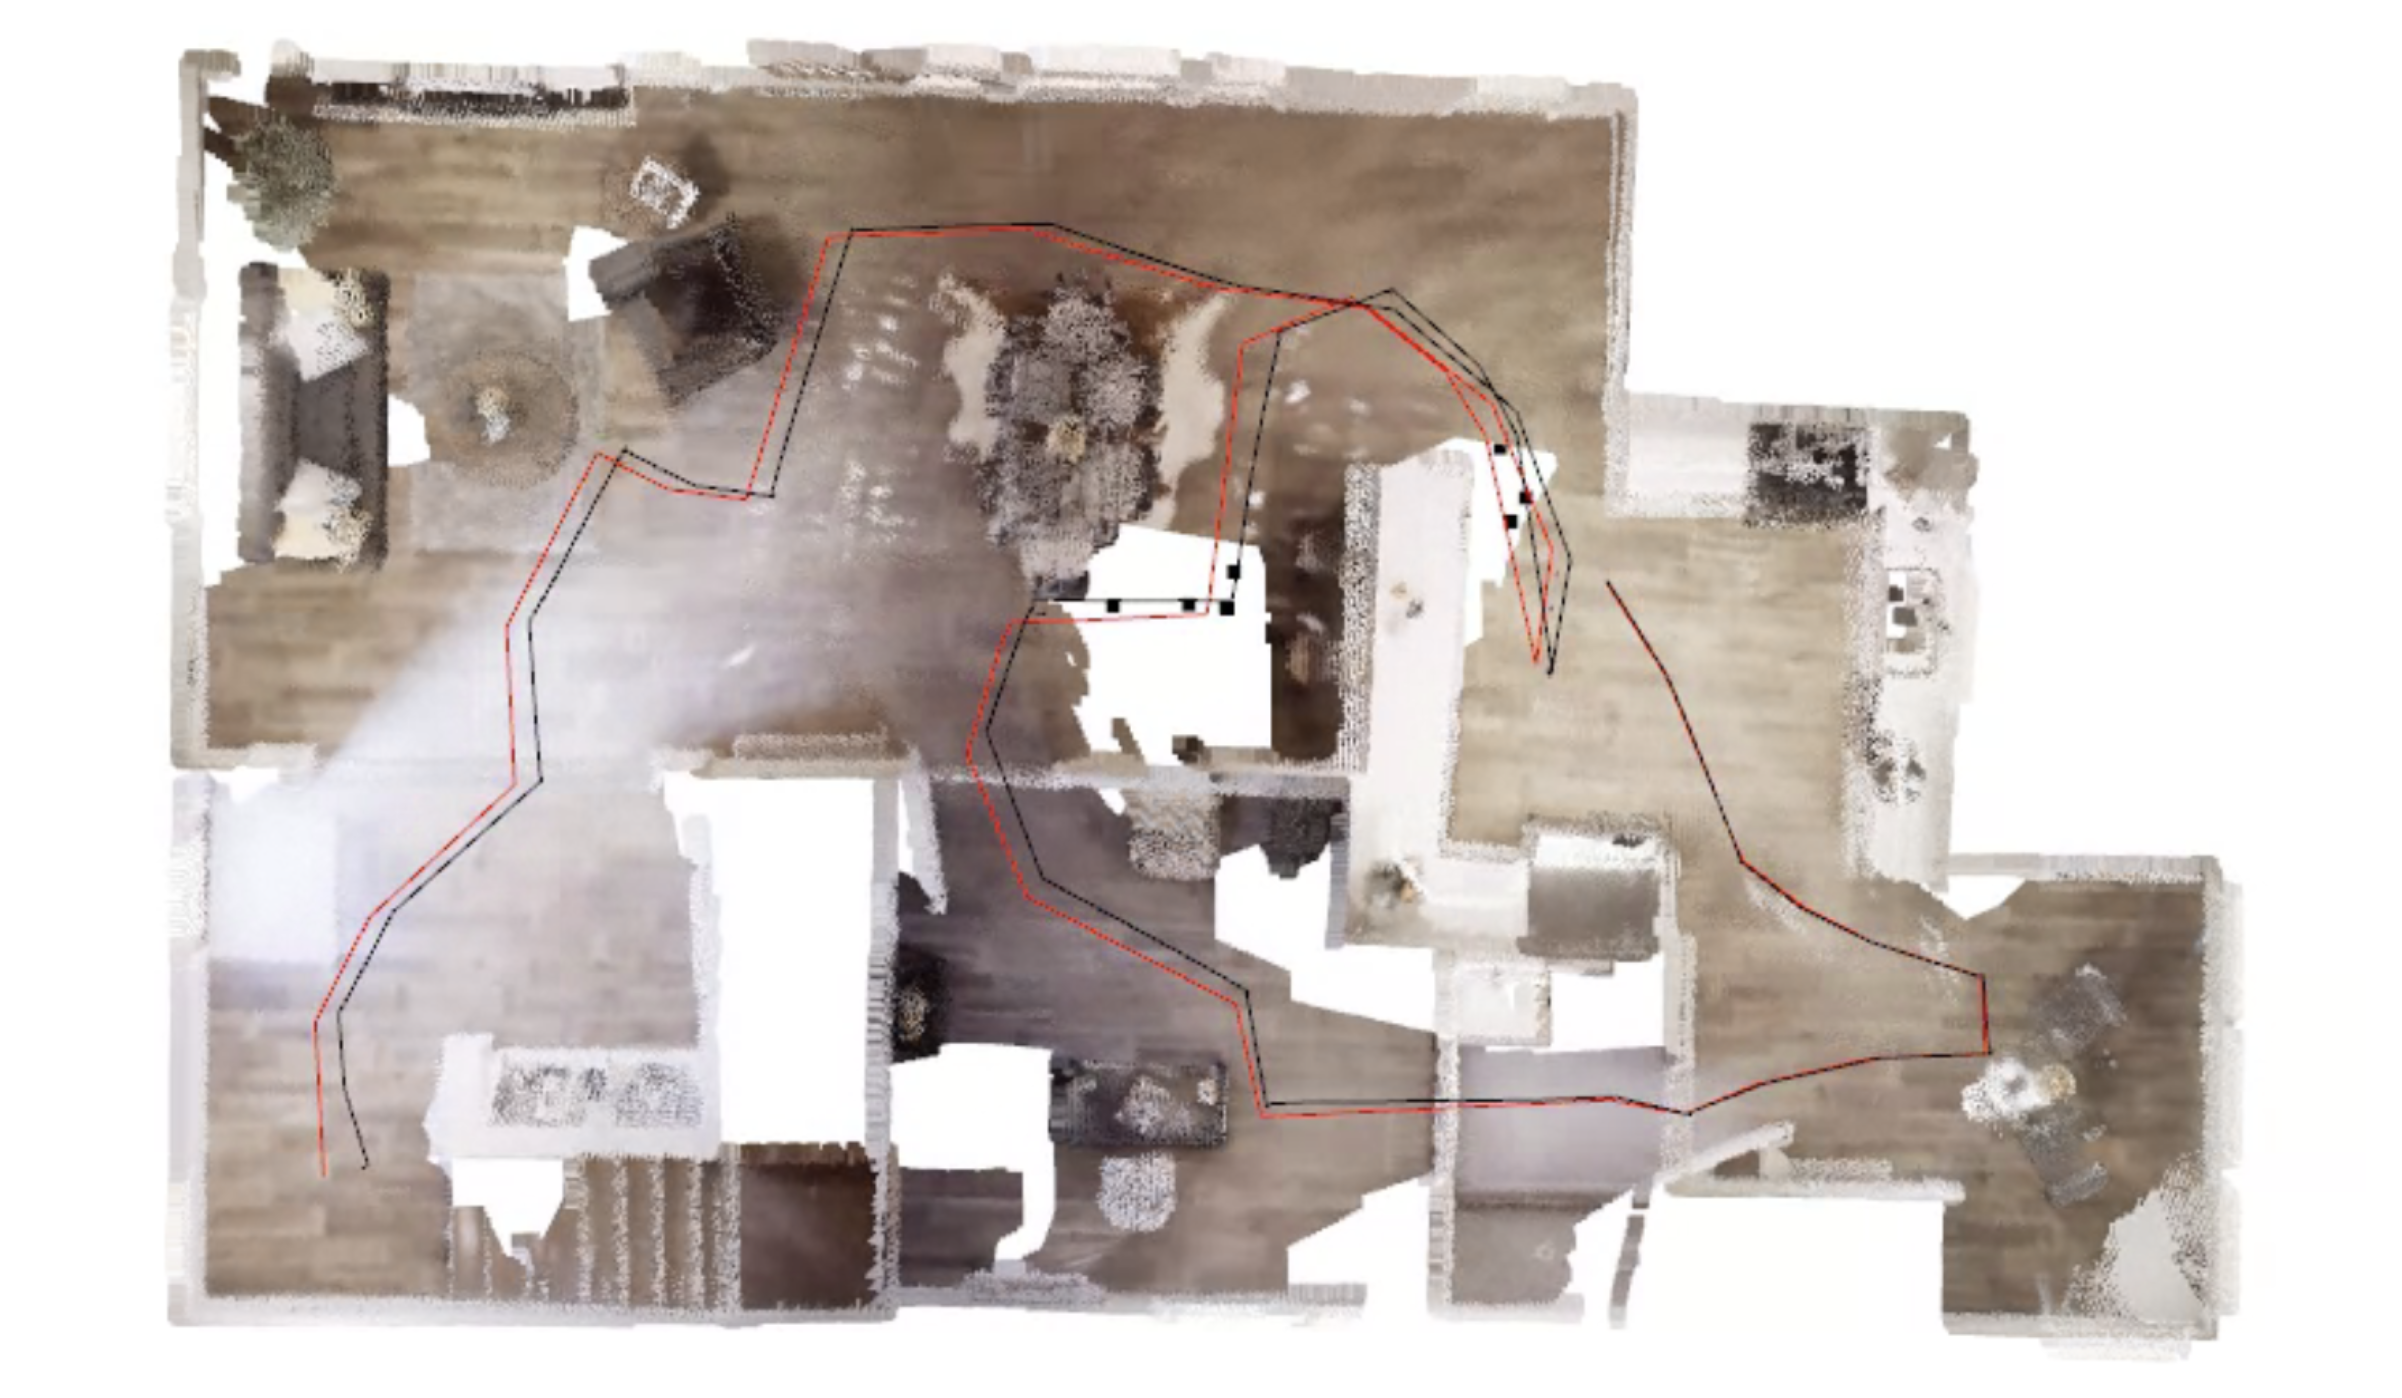
\includegraphics[width=0.8\linewidth]{image5.png}

    % \vspace{0.5em}

    % 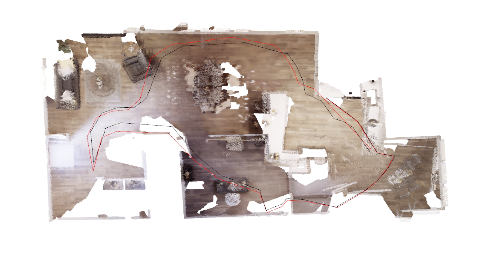
\includegraphics[width=0.5\linewidth]{image6.png}
    \caption{Reference first-floor reconstruction results (data size 152). The red and black lines show the estimated and ground-truth trajectories.}
    \label{fig:phase1-reference-results}
\end{figure}

\subsection{Phase 2: Second Floor Reconstruction}
Phase 2 uses the provided data-collection driver \code{hw1/load.py} to collect RGB-D observations and camera poses on the second floor of apartment\_0.

Its default configuration is \code{second_floor.yaml} under \code{hw1/configs/}. The simulator package is under \code{hw1/packages/simulator/}. From the repository root, run:
\begin{lstlisting}[language=bash]
pixi run -e habitat python load.py \\
  --config hw1/configs/second_floor.yaml \\
  --output-root eval/_data/second_floor/<student-id>
\end{lstlisting}
Use \code{w}/\code{s} to move, \code{a}/\code{d} to turn, \code{c} or Space to capture a frame, and \code{q} or Escape to finish. The more detailed controls and troubleshooting notes are in \code{hw1/docs/load.md}. The collector writes the following structure:
\begin{lstlisting}
<phase2-capture-dir>/
|-- rgb/<integer-stem>.png       # 8-bit color image (PNG)
|-- depth/<same-stem>.png        # 16-bit depth in millimeters; 0 = invalid
|-- GT_pose.npy                  # NumPy array, shape (N, 7)
`-- intrinsics.json              # JavaScript Object Notation (JSON)
\end{lstlisting}
The Phase 2 capture should contain synchronized RGB images, depth images, and camera poses. Record the output directory, route, frame count, and collection settings in \code{README.md}; do not submit the Replica environment assets themselves. Once the collector is configured, follow the workflow below:

\begin{enumerate}
\item Use the configured Habitat-Sim collector to navigate around the second floor of apartment\_0 and collect synchronized RGB images, depth images, and camera poses.
\item Run the same Standard Track reconstruction and evaluate the trajectory using Mean L2 Distance.
\item Measure and inspect the quality factors, preserving their values, settings, and links to relevant frames or pairs.
\item Compare Phase 2 with Phase 1 and discuss how coverage, viewpoint spacing, data quality, and algorithm parameters influenced reconstruction.
\end{enumerate}

\begin{figure}[htbp]
\centering
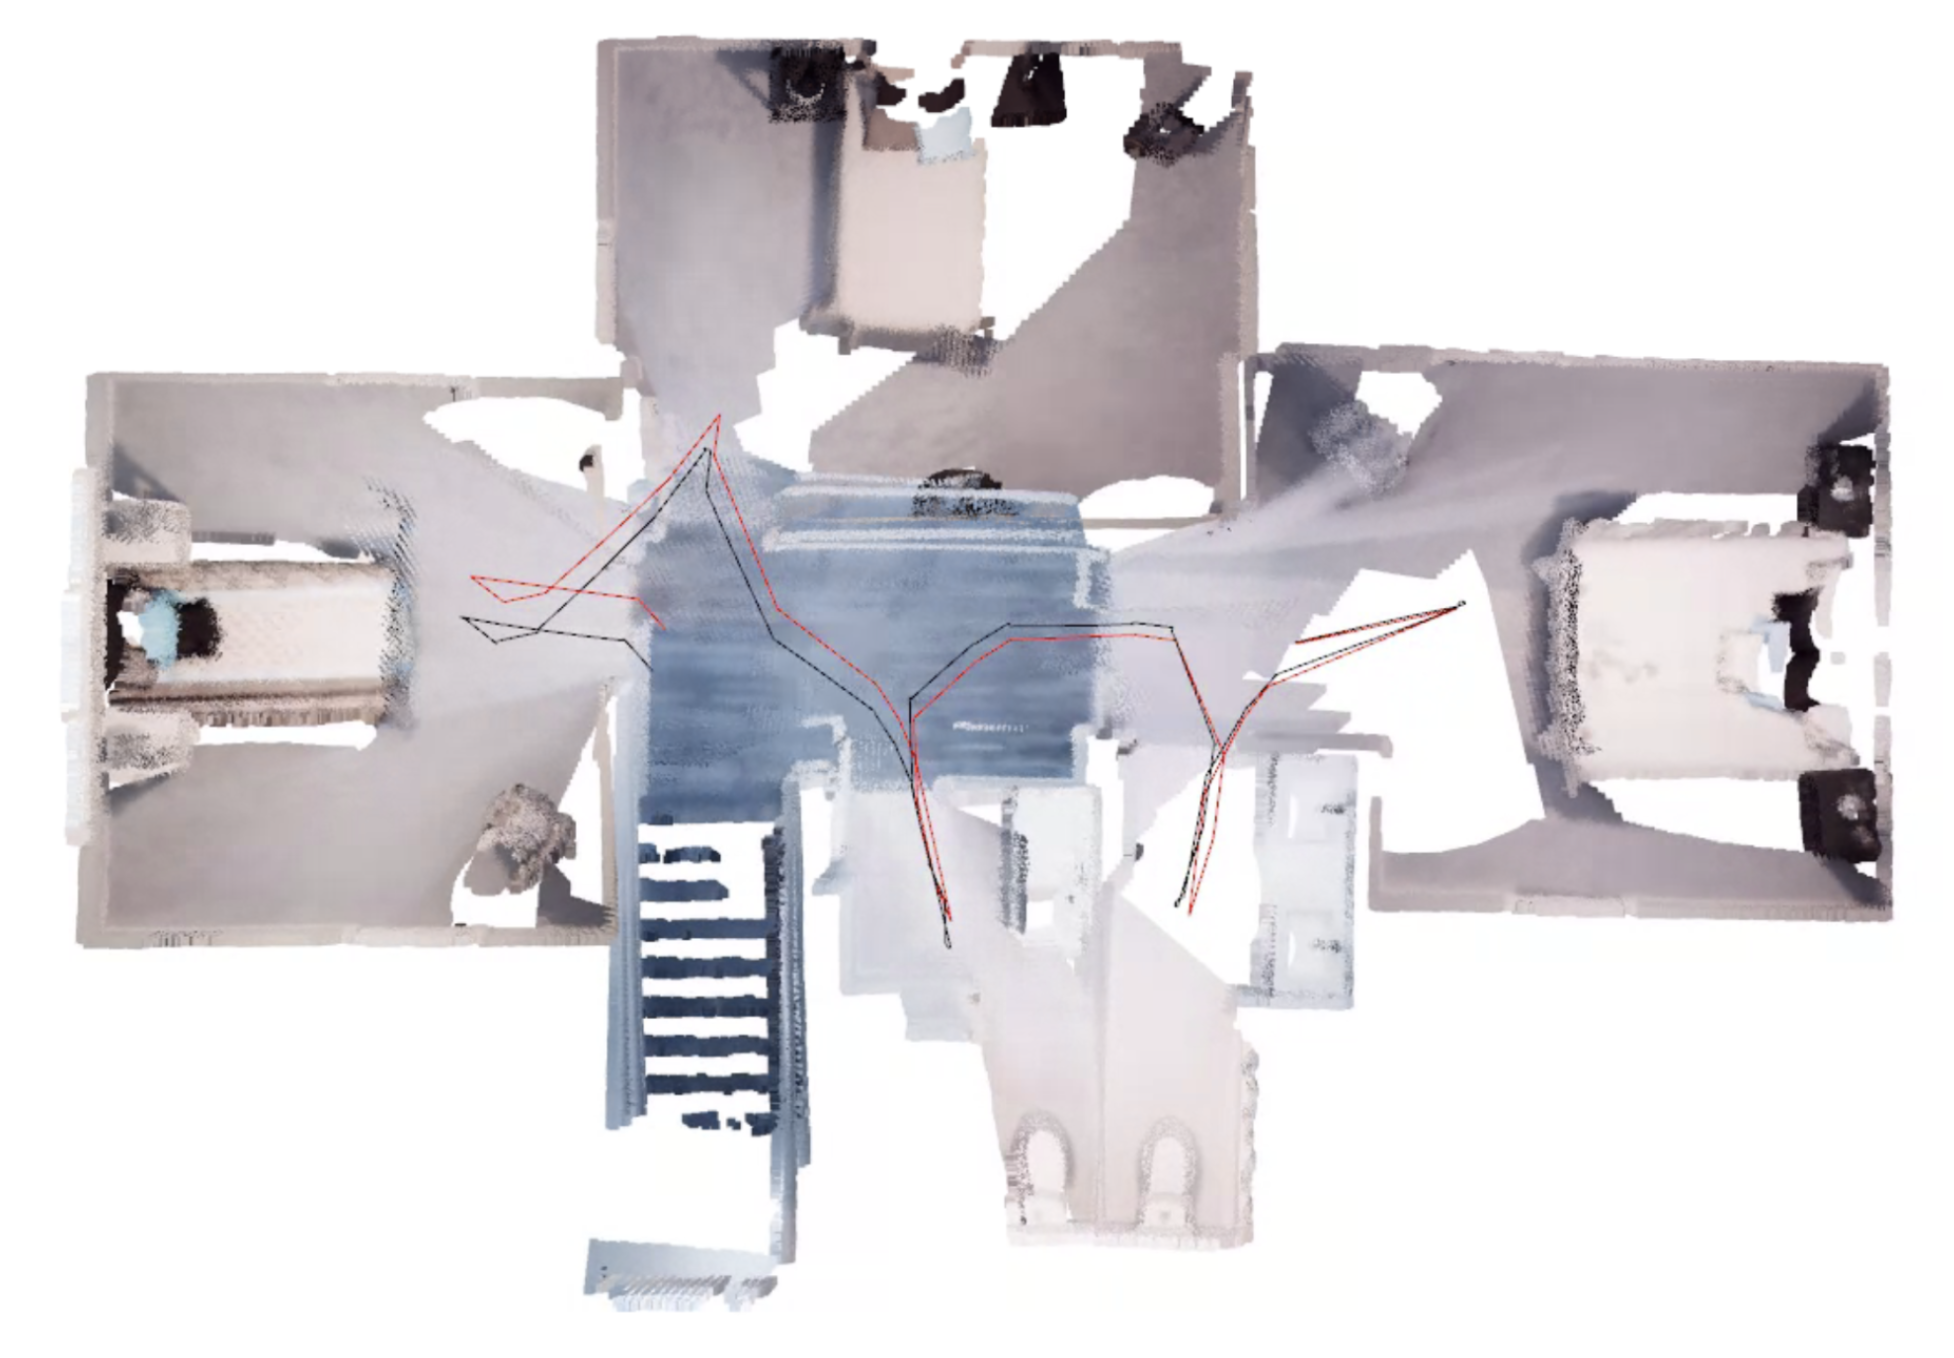
\includegraphics[width=0.8\linewidth]{image7.png}
\caption{Reference second-floor reconstruction result (data size 213). The red and black lines show the estimated and ground-truth trajectories.}
\label{fig:phase2-reference-result}
\end{figure}

\subsection{Optional Bonus: Custom ICP Implementation}
Implement \code{my_local_icp_algorithm} with nearest-neighbor correspondence
search and rigid transformation estimation. Compare its reconstruction results
and runtime with the Open3D-based ICP implementation to earn bonus points. The optional bonus is separate from the base score.

% ============================================================
% \section{Environment Setup and Resources}
% \subsection{Pixi installation}
% Pixi manages the repository's software environment. Install it using the official instructions for your operating system, then restart the shell so its executable is available on the system path \cite{pixiinstall}.
% \begin{lstlisting}[language=bash]
% curl -fsSL https://pixi.sh/install.sh | sh
% # Or use the official package-manager instructions for your platform.
% \end{lstlisting}

% \subsection{Repository setup}
% The main support target is 64-bit Linux. Habitat-Sim and the course workflow are configured and verified primarily on Linux. macOS and Windows with WSL may be used for development, but platform-specific graphics or binary differences may require additional adjustments.

% \smallskip
% \noindent\textbf{Linux.}
% Clone the course repository and install its Habitat environment from the repository root:
% \begin{lstlisting}[language=bash]
% git clone --recurse-submodules https://github.com/HCIS-Lab/physicalai26-hw.git
% cd physicalai26-hw/hw1
% pixi install -e habitat
% pixi run -e habitat python -c "import open3d, rdflib; print('ready')"
% \end{lstlisting}

% \smallskip
% \noindent\textbf{macOS.}
% Install Pixi using the official macOS guide \cite{pixiinstall}. Clone the repository as above and attempt \code{pixi install -e habitat} using the Habitat-Sim installation guidance \cite{habitatsiminstall}. Linux remains the primary platform; if simulator binaries or visualization dependencies are unavailable, use Linux or WSL.

% \smallskip
% \noindent\textbf{Windows with WSL.}
% Install WSL2 with Ubuntu, then run Linux commands inside the WSL terminal. Keep the repository and datasets within the WSL Linux filesystem. Native Windows is not the main supported target \cite{microsoftwsl}.

% ============================================================
\section{Grading}
% ============================================================
The program implementation accounts for 30\% of the grade, and the report accounts for the remaining 70\%. An optional custom ICP implementation can earn up to 20 additional bonus points.

\subsection{Program Implementation (30\%)}

The submitted implementation is assessed based on the completeness and correctness of the required Open3D-based reconstruction, data-collection, and data-verification workflow, as well as reproducibility and source-code organization. Automated evaluation scripts may be used to verify required functionality and reproducibility. Also, reconstruction quality is evaluated from two complementary aspects:
\begin{itemize}
    \item \textbf{Camera Trajectory Agreement: }
    The Mean L2 Distance measures the positional difference between the estimated and ground-truth camera trajectories. A lower value indicates closer agreement with the ground truth.

    \item \textbf{Scene Coverage and Completeness: }
    The reconstructed map should provide sufficient coverage of the target floor,
    including its major rooms, connecting spaces, and relevant corners, rather
    than reconstructing only a limited portion of the environment.
\end{itemize}

% The submitted program is assessed based on the required Open3D reconstruction, data collection and verification workflow, reproducibility, and source organization. The Standard Track is the complete base implementation. The optional Bonus Track is assessed from the submitted custom ICP implementation, its reconstruction result, and its documented comparison with the Open3D version.

\subsection{Report (70\%)}
% \begin{center}
% \begin{tabular}{L{0.58\linewidth} r}
% \toprule
% \textbf{Criterion} & \textbf{Weight} \\
% \midrule
% Pipeline implementation and data verification & 40\% \\
% Results, Mean L2 evaluation, visualizations, and discussion & 20\% \\
% Questions and technical analysis & 10\% \\
% \midrule
% Report total & 70\% \\
% \midrule
% Program implementation (submitted code) & 30\% \\
% Base score total & 100\% \\
% Optional custom ICP bonus & +20\% \\
% \bottomrule
% \end{tabular}
% \end{center}

The report should be submitted as a PDF, written in English, and kept concise.
It should include the following content:

\begin{itemize}

    \item \textbf{Methodology and Data Verification (30\%)}
    \begin{itemize}

        \item \textbf{Reconstruction Pipeline}
        \begin{itemize}
            \item Explain the implementation of each major reconstruction step.
            \item Describe the settings and parameter choices used in the pipeline.
            \item Discuss implementation issues encountered, the solutions used
            to address them, and the rationale behind those choices.
        \end{itemize}

        \item \textbf{Data Verification}
        \begin{itemize}
            \item Report the required data-quality measurements, measurement
            settings, and source links.
            \item Identify relevant failure cases and explain how the observed
            evidence relates to reconstruction artifacts or alignment failures.
            \item Describe any preprocessing or reconstruction adjustments made
            based on the analysis.
        \end{itemize}

    \end{itemize}

    \item \textbf{Results and Discussion (30\%)}
    \begin{itemize}
        \item Present reconstruction results for both phases.
        \item Provide reconstruction screenshots with the ceiling removed when
        needed, the estimated trajectory in red, and the ground-truth trajectory
        in black.
        \item Provide a comparison table for the reconstructions being compared,
        including:
        \begin{itemize}
            \item Mean L2 Distance;
            \item Evaluated frame count;
            \item Total execution time;
            \item Tested hyperparameters.
        \end{itemize}
        \item Compare the two phases and discuss the main findings based on both
        reconstruction results and data-verification evidence.
    \end{itemize}

    The Mean L2 Distance is required for each reconstruction being compared and
    should not be replaced by root mean square error, mean absolute error, or a
    metric computed after an additional fitted alignment.

    \item \textbf{Questions (10\%)}
    \begin{enumerate}
        \item What happens if ICP is performed without global registration
        (RANSAC)? Why?

        \item Describe the choices used to improve ICP stability, such as voxel
        size, correspondence thresholds, or robust losses.

        \item How do the observed data-quality factors and collection choices
        relate to reconstruction performance and Mean L2 Distance?
    \end{enumerate}

\end{itemize}

% \subsection{Questions}
% Answer the following questions in the report:
% \begin{enumerate}
% \item What happens if you perform ICP without global registration (RANSAC)? Why?
% \item Describe any choices used to improve ICP stability, such as voxel size, correspondence thresholds, or robust losses.
% \item How did the observed data-quality factors and collection choices affect the reconstruction and its Mean L2 Distance?
% \end{enumerate}

\subsection{Optional Bonus (+20\%)}
The optional bonus is assessed based on both the implementation of \code{my_local_icp_algorithm} and its evaluation in the report. Submit the corresponding source code and include a comparison with the Open3D-based ICP implementation, including reconstruction results, runtime, and implementation choices. Full bonus credit requires both the implementation, reconstruction quality, and the corresponding analysis in the report.

% ============================================================

% ============================================================
\section{Submission}
% ============================================================
\subsection{Submission Package}
Please submit \code{<student-id>_hw1.zip} to the designated submission platform. Please use the following structure at the zip root and avoid adding an extra enclosing directory:
\begin{lstlisting}
<student-id>_hw1.zip
|-- load.py
|-- reconstruct.py
|-- utils.py
|-- api.py
|-- ontology/
|   `-- hw1.ttl
|-- report.pdf
`-- README.md
\end{lstlisting}

Please include the source files used by the submitted reconstruction and verification pipeline. If you implement the optional bonus, please include the implementation of \code{my_local_icp_algorithm} in the submitted source and identify it in \code{README.md}; the bonus code should not replace or break the required Open3D path. Experiment declaration Turtle files, generated diagnostics, and the Phase 2 capture directory need not be included. Please include the report and omit the large Replica environment archive and unrelated build artifacts.

% \subsection{Report Contents}
% The report should be a PDF file written in English and should include:
% \begin{itemize}
% \item Discuss the results of every required pipeline step and the data-verification workflow, and share your findings;
% \item A concise explanation of the issues encountered during implementation, the solutions used to address them, and the justification for those choices;
% \item Reconstruction screenshots for both phases, with the ceiling removed when needed, the estimated trajectory in red, and the GT trajectory in black;
% \item A comparison table reporting the Mean L2 Distance for every reconstruction being compared, together with the evaluated frame count, unit, total execution time, and tested hyperparameters. The Mean L2 Distance is required for every reconstruction and may not be replaced by root mean square error, mean absolute error, or a metric based on an additional fitted alignment;
% \item The data-quality measurements, settings, source links, failure cases, and a discussion of how the evidence relates to reconstruction;
% \item Answers to the questions in the Assessment and Grading section;
% \item If the Bonus Track is attempted, a comparison of the custom ICP and Open3D results, runtime, and implementation choices.
% \end{itemize}

\subsection{Submission Rules}
Please observe the following submission rules:
\begin{itemize}
\item \textcolor{red}{Submission deadline: 2026/10/27 23:59}. The submission timestamp is determined by the designated submission platform.
\item An incorrect submission format or an extra top-level directory may result in a $-10$ point penalty.
\item Late submissions may receive a $-20$ point penalty per day.
\item Please submit original work. Plagiarism, including code or reports copied from other students or public repositories, is not permitted; confirmed plagiarism results in a score of zero.
\item Please write the report in English; a report written in another language receives a score of zero.
\end{itemize}
\printbibliography
\end{document}